% Tipo de documento e pacotes utilizados:
\documentclass{bmvc2k}

% Pacotes adicionais para documentos em português:
\usepackage[utf8]{inputenc}

% Outros pacotes que talvez venham a ser necessários:
\usepackage{subfigure}
\usepackage{url}

% Definição de macros:
\def\eg{\emph{e.g}\bmvaOneDot}
\def\Eg{\emph{E.g}\bmvaOneDot}
\def\etal{\emph{et al}\bmvaOneDot}

%-------------------------------------------------------------------------
% Título:
\title{Seletor de cores em imagens, arquivos de vídeo e entradas de vídeo.}

\addauthor{André Filipe Caldas Laranjeira\\ Matrícula: 16/0023777}{andrecaldaslaranjeira@gmail.com}{1}

\addinstitution{
  Departamento de Ciência da Computação\\
  Universidade de Brasília\\
  Campus Darcy Ribeiro, Asa Norte\\
  Brasília-DF, CEP 70910-900, Brazil
}

\runninghead{André, Laranjeira}{Projeto 01 -- Visão computacional -- \today}

%-------------------------------------------------------------------------
% Início do documento:
\begin{document}

\maketitle

%-------------------------------------------------------------------------
% Resumo:
\begin{abstract}
  Este relatório visa descrever o projeto de um programa seletor de cores, o qual permite ao usuário selecionar uma cor em uma imagem, arquivo de vídeo ou entrada de vídeo por meio de um clique do mouse. O programa utiliza as coordenadas do pixel em que o usuário clicou para extrair os valores em escala de cinzas ou escala BGR daquele pixel e destaca os pixels na imagem com cor parecida. Concluiu-se que esse programa é efetivo em mostrar ao usuário quais pixels de uma imagem, vídeo ou entrada de vídeo se assemelham em cor ao pixel escolhido.
\end{abstract}

%-------------------------------------------------------------------------
% Introdução:
\section{Introdução}

Uma imagem é um conjunto de pixels. Cada pixel é representado por um valor de 0 a 255 em imagens em escala de cinzas ou por 3 valores de 0 a 255 em imagens coloridas que utilizam a escala RGB ou a escala BGR (um para a cor azul, outro para a cor verde e o outro para a cor vermelha). A semelhança entre a cor de um par de pixels está expressa em quão pequena é a distância entre os valores utilizados para representar a cor de cada um desses pixels. Um vídeo, por sua vez, é um conjunto de imagens (denominadas frames) exibidas em certa velocidade (geralmente, 30 frames por segundo). Cada frame é, portanto, formado por um conjunto de pixels, assim como uma imagem.

O projeto demonstrativo criado visa permitir ao usuário escolher um pixel de uma imagem ou de um frame de um vídeo com um clique de mouse, exibir as informações da posição daquele pixel na imagem ou frame de vídeo e dos valores de cor relativos aquele pixel e modificar a imagem ou os próximos frames do vídeo para destacar outros pixels com uma cor semelhante ao pixel selecionado. Isso permite ao usuário verificar com clareza quais pixels de uma imagem possuem cores semelhantes ao pixel selecionado e onde os pixels com cor semelhante se localizam.

%     Introdução: Apresentar de forma clara, porém sucinta, os objetivos do projeto demonstrativo. Deve conter também uma breve explanação dos conhecimentos básicos relacionado ao projeto e uma breve revisão bibliográfica relacionada ao problema. Utilize sempre fontes bibliográficas confiáveis (livros e artigos científicos), evitando utilizar única e exclusivamente fontes de baixa confiabilidade (Wikipédia, Stackoverflow,...).

%-------------------------------------------------------------------------
% Metodologia:
\section{Metodologia}
Para que o usuário possa interagir com a imagem ou vídeo, o programa utiliza-se dos métodos {\em imread} e {\em VideoCapture} de biblioteca {\bf OpenCV} para ler imagems e vídeos (tanto arquivos como o stream de vídeo de uma webcam), respectivamente ~\cite{OpenCV}. O programa então configura a janela de exibição do programa, uma variável global para cor selecionada e um método de {\em callback} para gerenciar eventos de mouse na janela. Para finalizar a configuração inicial, o programa o verifica se a imagem está em escala de cinzas ou não pelo {\em shape} do arquivo carregado.

Para utilizar o programa, o usuário deve clicar com o botão esquerdo do mouse em um pixel na imagem. Quando isso ocorre, um método de {\em callback} é chamado com as coordenadas x e y da imagem ou do frame em que o clique foi realizado sendo fornecidos como argumentos. Esse método então converte as coordenadas x e y na coluna e na linha da imagem ou do frame de vídeo, encontra a cor utilizada na imagem ou no frame naquele ponto e imprime essas informações para o usuário. Por fim, esse método salva as informações de cor em uma variável global para que elas possam ser acessadas na função principal.

Em um certo intervalo de tempo, o laço principal do programa verifica se alguma cor foi selecionada pelo usuário. Quando isso ocorre, o programa chama um método para destacar os pixels da imagem ou do próximo frame do vídeo que possuam cor semelhante. Esse método utiliza várias funções do pacote {\em numpy} e possui um funcionamento relativamente complicado. Primeiro, se gera uma cópia da imagem ou do frame. Então, uma matriz com a distância ao quadrado entre cada componente de cor do pixel da imagem ou do frame em relação à cada componente de cor da cor escolhida é gerada. Com essa matriz de distâncias ao quadrado, se calcula uma máscara que aponta os pixels da imagem ou do frame cuja distância euclidiana até a cor escolhida é menor que um certo valor (no caso desse programa, 13). Por fim, o método substitui na cópia da imagem ou do frame gerada no primeiro passo todos os pixels presentes na máscara pela cor branca em imagens de escala de cinzas e pela cor vermelha em imagens coloridas e retorna essa cópia modificada da imagem ou do frame. O laço principal do programa então exibe a imagem ou frame modificado para o usuário.

%     Metodologia: É dedicada a uma exposição dos métodos e procedimentos adotados no projeto demonstrativo.

%-------------------------------------------------------------------------
% Resultados:
\section{Resultados}
Os resultados obtidos foram satisfatórios tanto para imagens como para arquivos de vídeo, demarcando de forma clara os pixels da imagem que se assemelhavam ao pixel escolhido.

Na figura \ref{fig:image_test}, podemos visualizar um teste do programa na imagem "Atlas avatar.jpg", no qual o usuário apenas selecionou um pixel de uma imagem. A figura mostra a imagem antes e depois do usuário clicar em um pixel da imagem, bem como a saída do terminal identificando corretamente as informações do pixel escolhido pelo usuário.

\begin{figure}
    \centering
    \subfigure[Imagem antes do usuário selecionar o pixel da linha 28 e coluna 126.]{
        \centering
        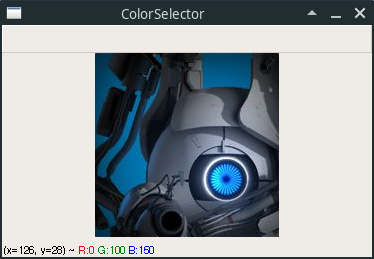
\includegraphics[scale=0.4]{Imagens/image_test_1.png}
        \label{fig:image_test_before}
    }
    \subfigure[Imagem após o usuário selecionar o pixel da linha 28 e coluna 126.]{
        \centering
        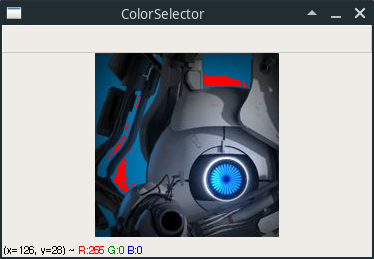
\includegraphics[scale=0.4]{Imagens/image_test_2.png}
        \label{fig:image_test_after}
    }
    \subfigure[Saída do terminal após o usuário selecionar o pixel da linha 28 e coluna 126.]{
        \centering
        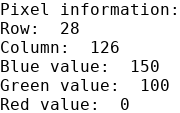
\includegraphics[scale=0.65]{Imagens/image_test_3.png}
        \label{fig:image_test_output}
    }
    \caption{Teste realizado com a imagem "Atlas avatar.jpg".}
    \label{fig:image_test}
\end{figure}

Já na figura \ref{fig:video_test}, podemos visualizar um teste do programa no vídeo "Cargo test.avi", mostrando um conjunto de frames que destaca uma única cor escolhida pelo usuário. Note que, com o decorrer do vídeo, os pixels demarcados pelo programa vão sendo atualizados para manter em destaque a cor selecionada pelo usuário em um frame anterior do vídeo. Embora a utilização desse programa em arquivos de vídeo torne necessário que cada frame individual seja modificado, a execução do programa em arquivos de vídeo {\bf não} apresentou atraso perceptível ao usuário na execução do programa, o que pode ser explicado pela utilização do pacote {\em numpy}.

\begin{figure}
    \centering
    \subfigure[Primeiro frame destacando a cor selecionada pelo usuário.]{
        \centering
        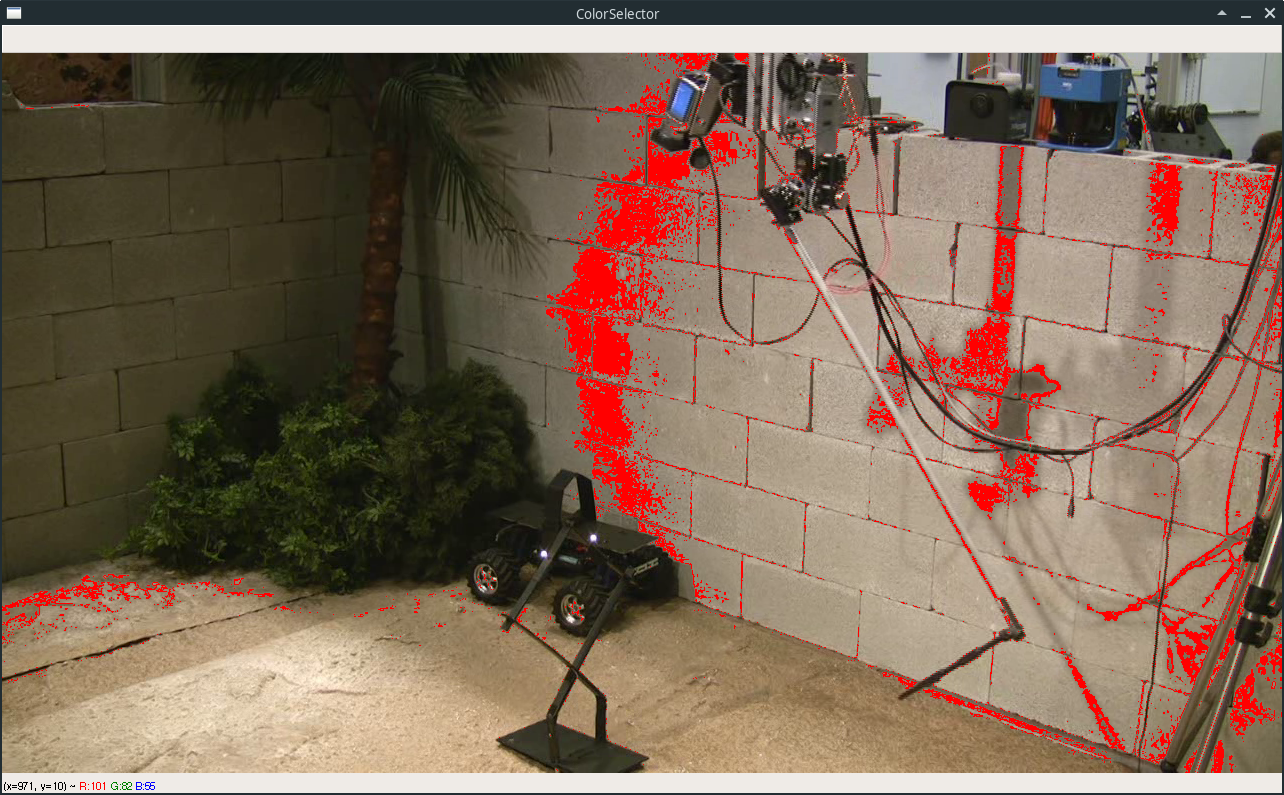
\includegraphics[scale=0.1]{Imagens/video_test_1.png}
        \label{fig:video_test_frame1}
    }
    \subfigure[Segundo frame destacando a cor selecionada pelo usuário.]{
        \centering
        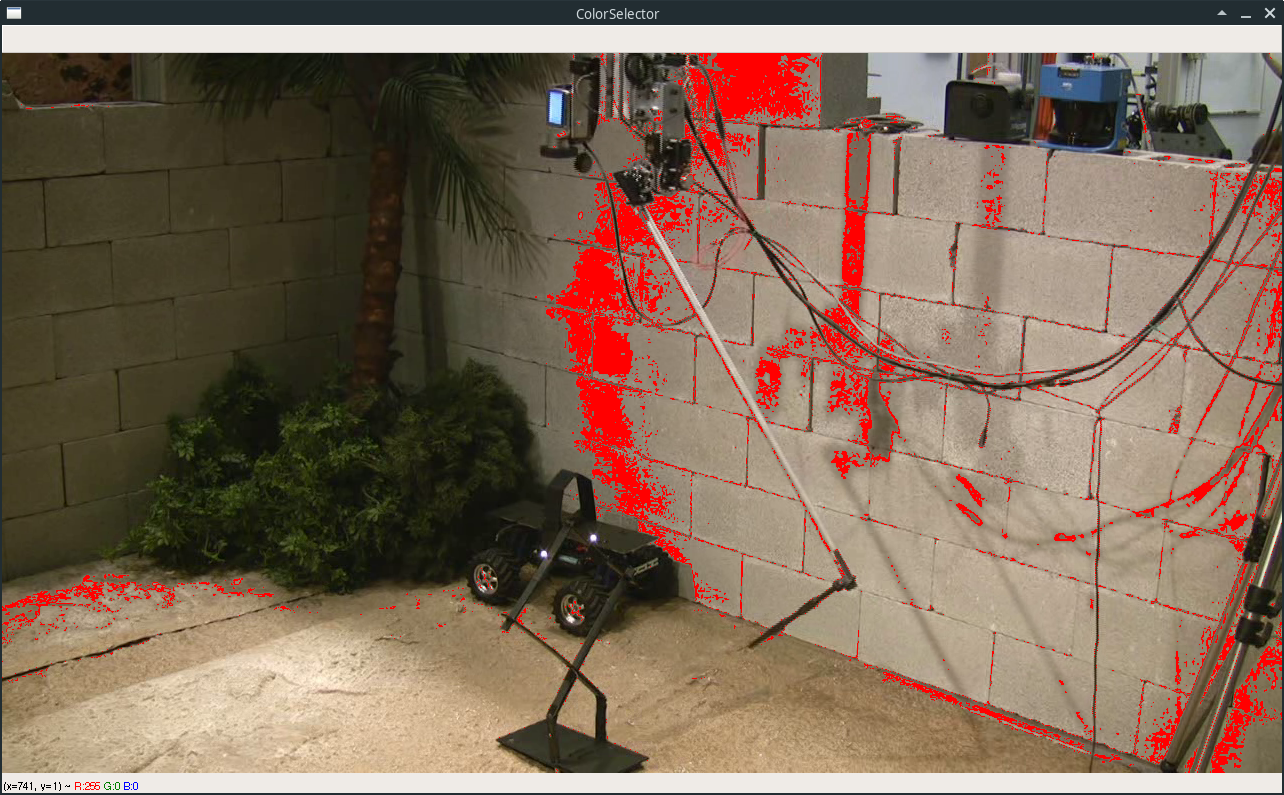
\includegraphics[scale=0.1]{Imagens/video_test_2.png}
        \label{fig:video_test_frame2}
    }
    \subfigure[Terceiro frame destacando a cor selecionada pelo usuário.]{
        \centering
        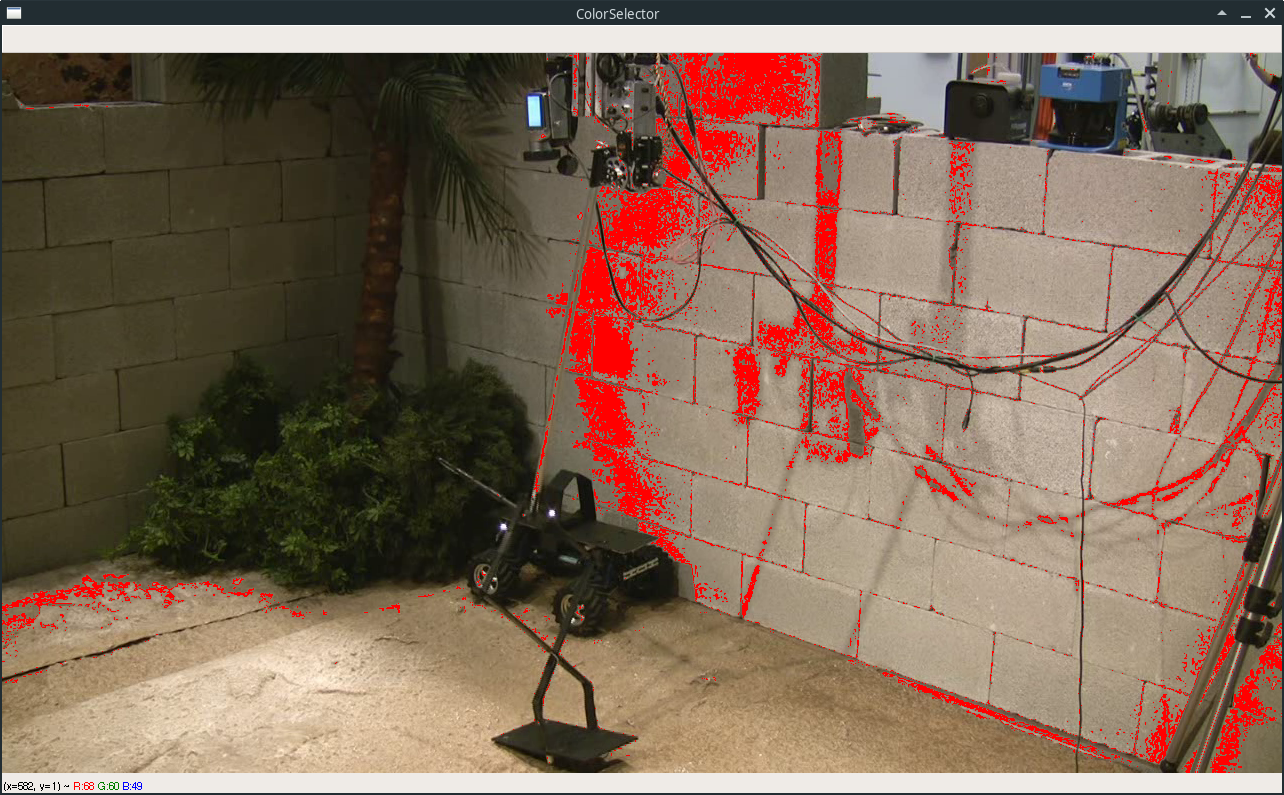
\includegraphics[scale=0.1]{Imagens/video_test_3.png}
        \label{fig:video_test_frame3}
    }
    \caption{Teste realizado com o arquivo de vídeo "Cargo test.avi".}
    \label{fig:video_test}
\end{figure}

%     Resultados: Nessa parte são apresentados os resultados das implementações efetuadas, na forma de tabelas e figuras, sem se esquecer de identificar em cada caso os parâmetros utilizados. Rotule todos os eixos dos gráficos apresentados. Caso o projeto demonstrativo tenha vários requisitos independentes, você pode criar uma seção para cada requisito e apresentar subseções de metodologia e resultados para cada um.

%-------------------------------------------------------------------------
% Conclusões:
\section{Conclusões}
Com base nos resultados obtidos, podemos constatar que o projeto demonstrativo atingiu o objetivo teórico com sucesso, apresentando a funcionalidade adequada. Por meio desse projeto, foi possível aprender os conceitos básicos relacionados à biblioteca {\bf OpenCV} com a criação de um programa capaz de selecionar um pixel em uma imagem ou vídeo e destacar nessa mesma imagem ou nos próximos frames do vídeo todos os pixels com uma cor semelhante à cor do pixel selecionado. Além disso, a utilização do pacote {\em numpy} permitiu que o programa fosse executado sem atraso perceptível ao usuário.

%     Discussão e Conclusões: A discussão visa comparar os resultados obtidos e os previstos pela teoria. Deve-se justificar eventuais discrepâncias observadas. As conclusões resumem a atividade e destacam os principais resultados e aplicações dos conceitos vistos.

%     Bibliografia: Citar as fontes consultadas, respeitando as regras de apresentação de bibliografia (autor, título, editora, edição, ano, página de início e fim). Inclua o máximo possível de informações nas referências, por exemplo, inclua todos os autores e evite o uso de "et al." na lista de referências. No caso de citação de página da web, tente identificar seus autores e data da última atualização. Somente quando tais informações não estão disponíveis, indique a data em que você visitou a página.

\bibliography{refs}
\end{document}

%-------------------------------------------------------------------------
% Lembrete da estrutura:
%
% Deverá conter as seguintes partes:
%
%     Identificação: Possuir a indicação clara do título do projeto demonstrativo abordado, nome do(s) autor(es), e quando houver, número(s) de matrícula e e-mail(s).
%     Resumo: Breve resumo do projeto e das suas conclusões.
%     Introdução: Apresentar de forma clara, porém sucinta, os objetivos do projeto demonstrativo. Deve conter também uma breve explanação dos conhecimentos básicos relacionado ao projeto e uma breve revisão bibliográfica relacionada ao problema. Utilize sempre fontes bibliográficas confiáveis (livros e artigos científicos), evitando utilizar única e exclusivamente fontes de baixa confiabilidade (Wikipédia, Stackoverflow,...).
%     Metodologia: É dedicada a uma exposição dos métodos e procedimentos adotados no projeto demonstrativo.
%     Resultados: Nessa parte são apresentados os resultados das implementações efetuadas, na forma de tabelas e figuras, sem se esquecer de identificar em cada caso os parâmetros utilizados. Rotule todos os eixos dos gráficos apresentados. Caso o projeto demonstrativo tenha vários requisitos independentes, você pode criar uma seção para cada requisito e apresentar subseções de metodologia e resultados para cada um.
%     Discussão e Conclusões: A discussão visa comparar os resultados obtidos e os previstos pela teoria. Deve-se justificar eventuais discrepâncias observadas. As conclusões resumem a atividade e destacam os principais resultados e aplicações dos conceitos vistos.
%     Bibliografia: Citar as fontes consultadas, respeitando as regras de apresentação de bibliografia (autor, título, editora, edição, ano, página de início e fim). Inclua o máximo possível de informações nas referências, por exemplo, inclua todos os autores e evite o uso de "et al." na lista de referências. No caso de citação de página da web, tente identificar seus autores e data da última atualização. Somente quando tais informações não estão disponíveis, indique a data em que você visitou a página.
%
% O relatório deverá ser confeccionado em editor eletrônico de textos com no máximo 7 (sete) páginas (sem contar as referencias bibliográficas), utilizando obrigatoriamente o padrão de formatação descrito no arquivo de exemplo disponibilizado aqui, para processadores de texto LaTeX. Não serão permitidos relatórios confeccionados em outro processador de texto, ou usando um modelo diferente do padrão LaTeX disponibilizado.
